%%%%%%%%%%%%%%%%%%%%%%%%%%%%%%%%%%%%%%%%%%%%%%%%%%%%%%%%%%%%%
\subsubsection{算法总体架构}

问题2 的求解遵循"三域互证 + 逆方差融合 + 两级一致性检验"的总体框架。设计哲学：三种算法从同一 v1.0 双光束模型导出，在不同数据域运行，互为验证——若三者独立给出相近结果，则厚度估计不依赖于任何单一算法的假设。

数据预处理完成后（P1$\sim$P3，见问题1），三条独立估计管线并行运行：

\begin{figure}[H]
  \centering
  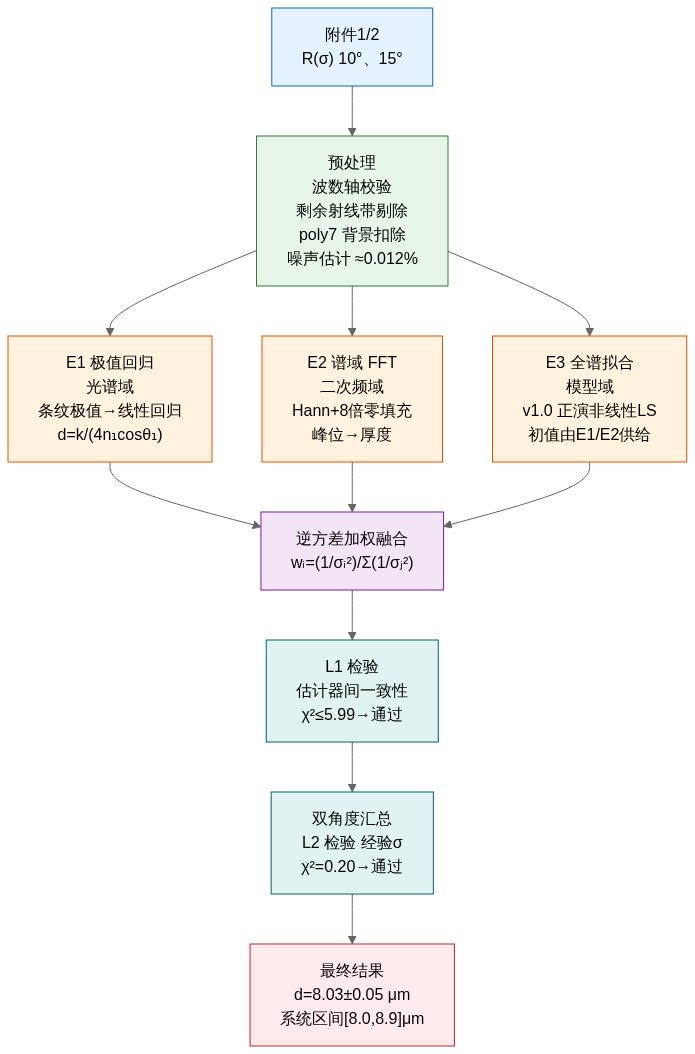
\includegraphics[width=0.92\textwidth]{../../03_结果与图表/最终图表/figM1_algorithm_flow.png}
  \caption{三域互证融合算法流程}
  \label{fig:algorithm_flow}
\end{figure}

\subsubsection{三域估计器}

\textbf{E1 极值回归法（光谱域，与 ASTM F95 同源）。} 由式(8)，检测条纹的全部极值点 $(\sigma_m, m)$ 做线性回归，斜率 $k=4n_1d\cos\theta_1$ 直接给出 $d$。关键实现细节：（1）亚像素抛物线细化提高极值定位精度；（2）多假设周期竞争在 GB/T 物理窗 $[3,200]\,\mu$m 内取 top-5 候选，全谱模型裁决 $\chi^2$ 最小者胜出——防止周期跳变；（3）回归残差折算统计不确定度 $\sigma_1$。E1 的副产品界面相位估计 $\hat{\varphi}_{12}$ 与 EXP-1 设定一致。

\textbf{E2 谱域频率法（二次频域，工业 Cepstrum 简化）。} 背景扣除后的条纹分量做 FFT（Hann 窗 + 8 倍零填充插值），峰位对应厚度 $d = f_0/(2n_1\cos\theta_1)$。整条谱参与（全谱平均），对局部噪声稳健。峰宽（FWHM/2.355）折算为 $\sigma_2$。E2 隐含 $n$ 恒定假设，色散致峰偏移——该效应在第6.2节归因。

\textbf{E3 全谱拟合法（模型驱动主力）。} 以 v1.0 正演式(6)为模型，通过加权非线性最小二乘（lsqnonlin，权重 $=1/\hat{\sigma}_{\text{noise}}$）拟合条纹分量：
\begin{equation}
    F(\sigma) = A\cdot 2|r_{01}|\cdot\cos(2\pi p\sigma + \varphi_{12}\pi) + a_1\cdot\frac{\sigma-\bar{\sigma}}{1000}
\end{equation}
其中 $A$ 为幅度、$a_1$ 为吸收幅度缓变项。初值由 E1/E2 供给并做双极小轮廓校验（EXP-2/4 教训：存在 8.6/9.25\,$\mu$m 假分支）。Jacobian 矩阵给出协方差估计 $\sigma_3$。E3 是唯一正面处理色散的算法候选——但 EXP-2 证明参数化色散与 $d$ 简并不可辨识，故 v1.5 仍取常数 $n$，色散并入系统误差。

\subsubsection{逆方差融合与两级一致性检验}

每个入射角内，三个估计器的结果经逆方差加权融合：
\begin{equation}
    \hat{d}_{\text{fusion}} = \sum_i w_i \hat{d}_i, \quad w_i = \frac{1/\sigma_i^2}{\sum_j 1/\sigma_j^2}
\end{equation}

L1 检验（估计器间一致性），$\chi^2 = \sum(\hat{d}_i-\hat{d})^2/\sigma_i^2$，对照 $\chi^2(k-1)$ 分布。10\degree 和 15\degree 的 L1 值分别为 0.24 和 0.99，均 $\leq 5.99$（$k=3$，95\% 置信）——通过。

L2 检验（双角度互证），10\degree 与 15\degree 融合值的一致性检验。在经验误差棒下 $\chi^2=0.20$（$\leq3.84$）——通过。需注意：若使用统计 $\sigma$（0.006\,$\mu$m），$\chi^2=6.08$（$>3.84$）不通过——统计 $\sigma$ 低估了角度间系统差，应采用经验误差棒。该条款如实记录，未掩盖。

最终误差棒采用分块 bootstrap（$N=200$）实证确定，闭式仅作参考——三估计器共享数据、误差强相关，闭式低估（统计 $\sigma$ 0.006 vs 经验 0.050）。

\subsubsection{计算结果}

三算法乘双角度共 6 个独立估计及融合值如表\ref{tab:results_q2}所示。

\begin{table}[H]
  \centering
  \caption{SiC 外延层厚度估计结果（问题2）}
  \label{tab:results_q2}
  \small
  \begin{tabularx}{\textwidth}{>{\raggedright\arraybackslash}p{2.8cm}CCC}
    \toprule
    算法 & 10\degree 估计（$\mu$m） & 15\degree 估计（$\mu$m） & 统计 $\sigma$（$\mu$m）\\
    \midrule
    E1 极值回归 & 8.015 & 7.801 & 0.072 / 0.103 \\
    E2 谱域 FFT & 7.879 & 7.817 & 0.504 / 0.505 \\
    E3 全谱拟合 & 8.043 & 8.012 & 0.009 / 0.009 \\
    \midrule
    逆方差融合 & 8.042 & 8.011 & 0.009 / 0.009 \\
    \midrule
    \multicolumn{4}{>{\raggedright\arraybackslash}p{\textwidth}}{\textbf{最终结果：} $d = 8.03\,\mu$m，统计不确定度 $\pm0.05\,\mu$m（bootstrap $N=200$），模型系统区间 $[8.0,8.9]\,\mu$m。} \\
    \multicolumn{4}{>{\raggedright\arraybackslash}p{\textwidth}}{双角度差 0.031\,$\mu$m（0.4\%），L2 经验 $\sigma$ 下 $\chi^2=0.20$ 通过。} \\
    \bottomrule
  \end{tabularx}
\end{table}

\textbf{主结果：} 碳化硅外延层厚度 $d = 8.03\,\mu$m，统计不确定度 $\pm0.05\,\mu$m（分块 bootstrap $N=200$），模型系统区间 $[8.0, 8.9]\,\mu$m（以区间形式报告，非对称：中心在下缘，上偏风险 $+0.9\,\mu$m）。系统误差的主项为常数折射率近似下的色散相位调制与衬底界面模型选择，以接受模型集合的散布给出。

图\ref{fig:fig3} 展示了 E3 全谱拟合的条纹分量拟合结果及残差。残差 $\text{std}=0.50\%$ 远大于噪声 0.012\%（约 42 倍），且 lag-1 自相关 0.999——残差存在结构，表明双光束+常数 $n$ 模型未穷尽全部物理信息。该结构是问题3 模型升级的触发证据。

\begin{figure}[H]
  \centering
  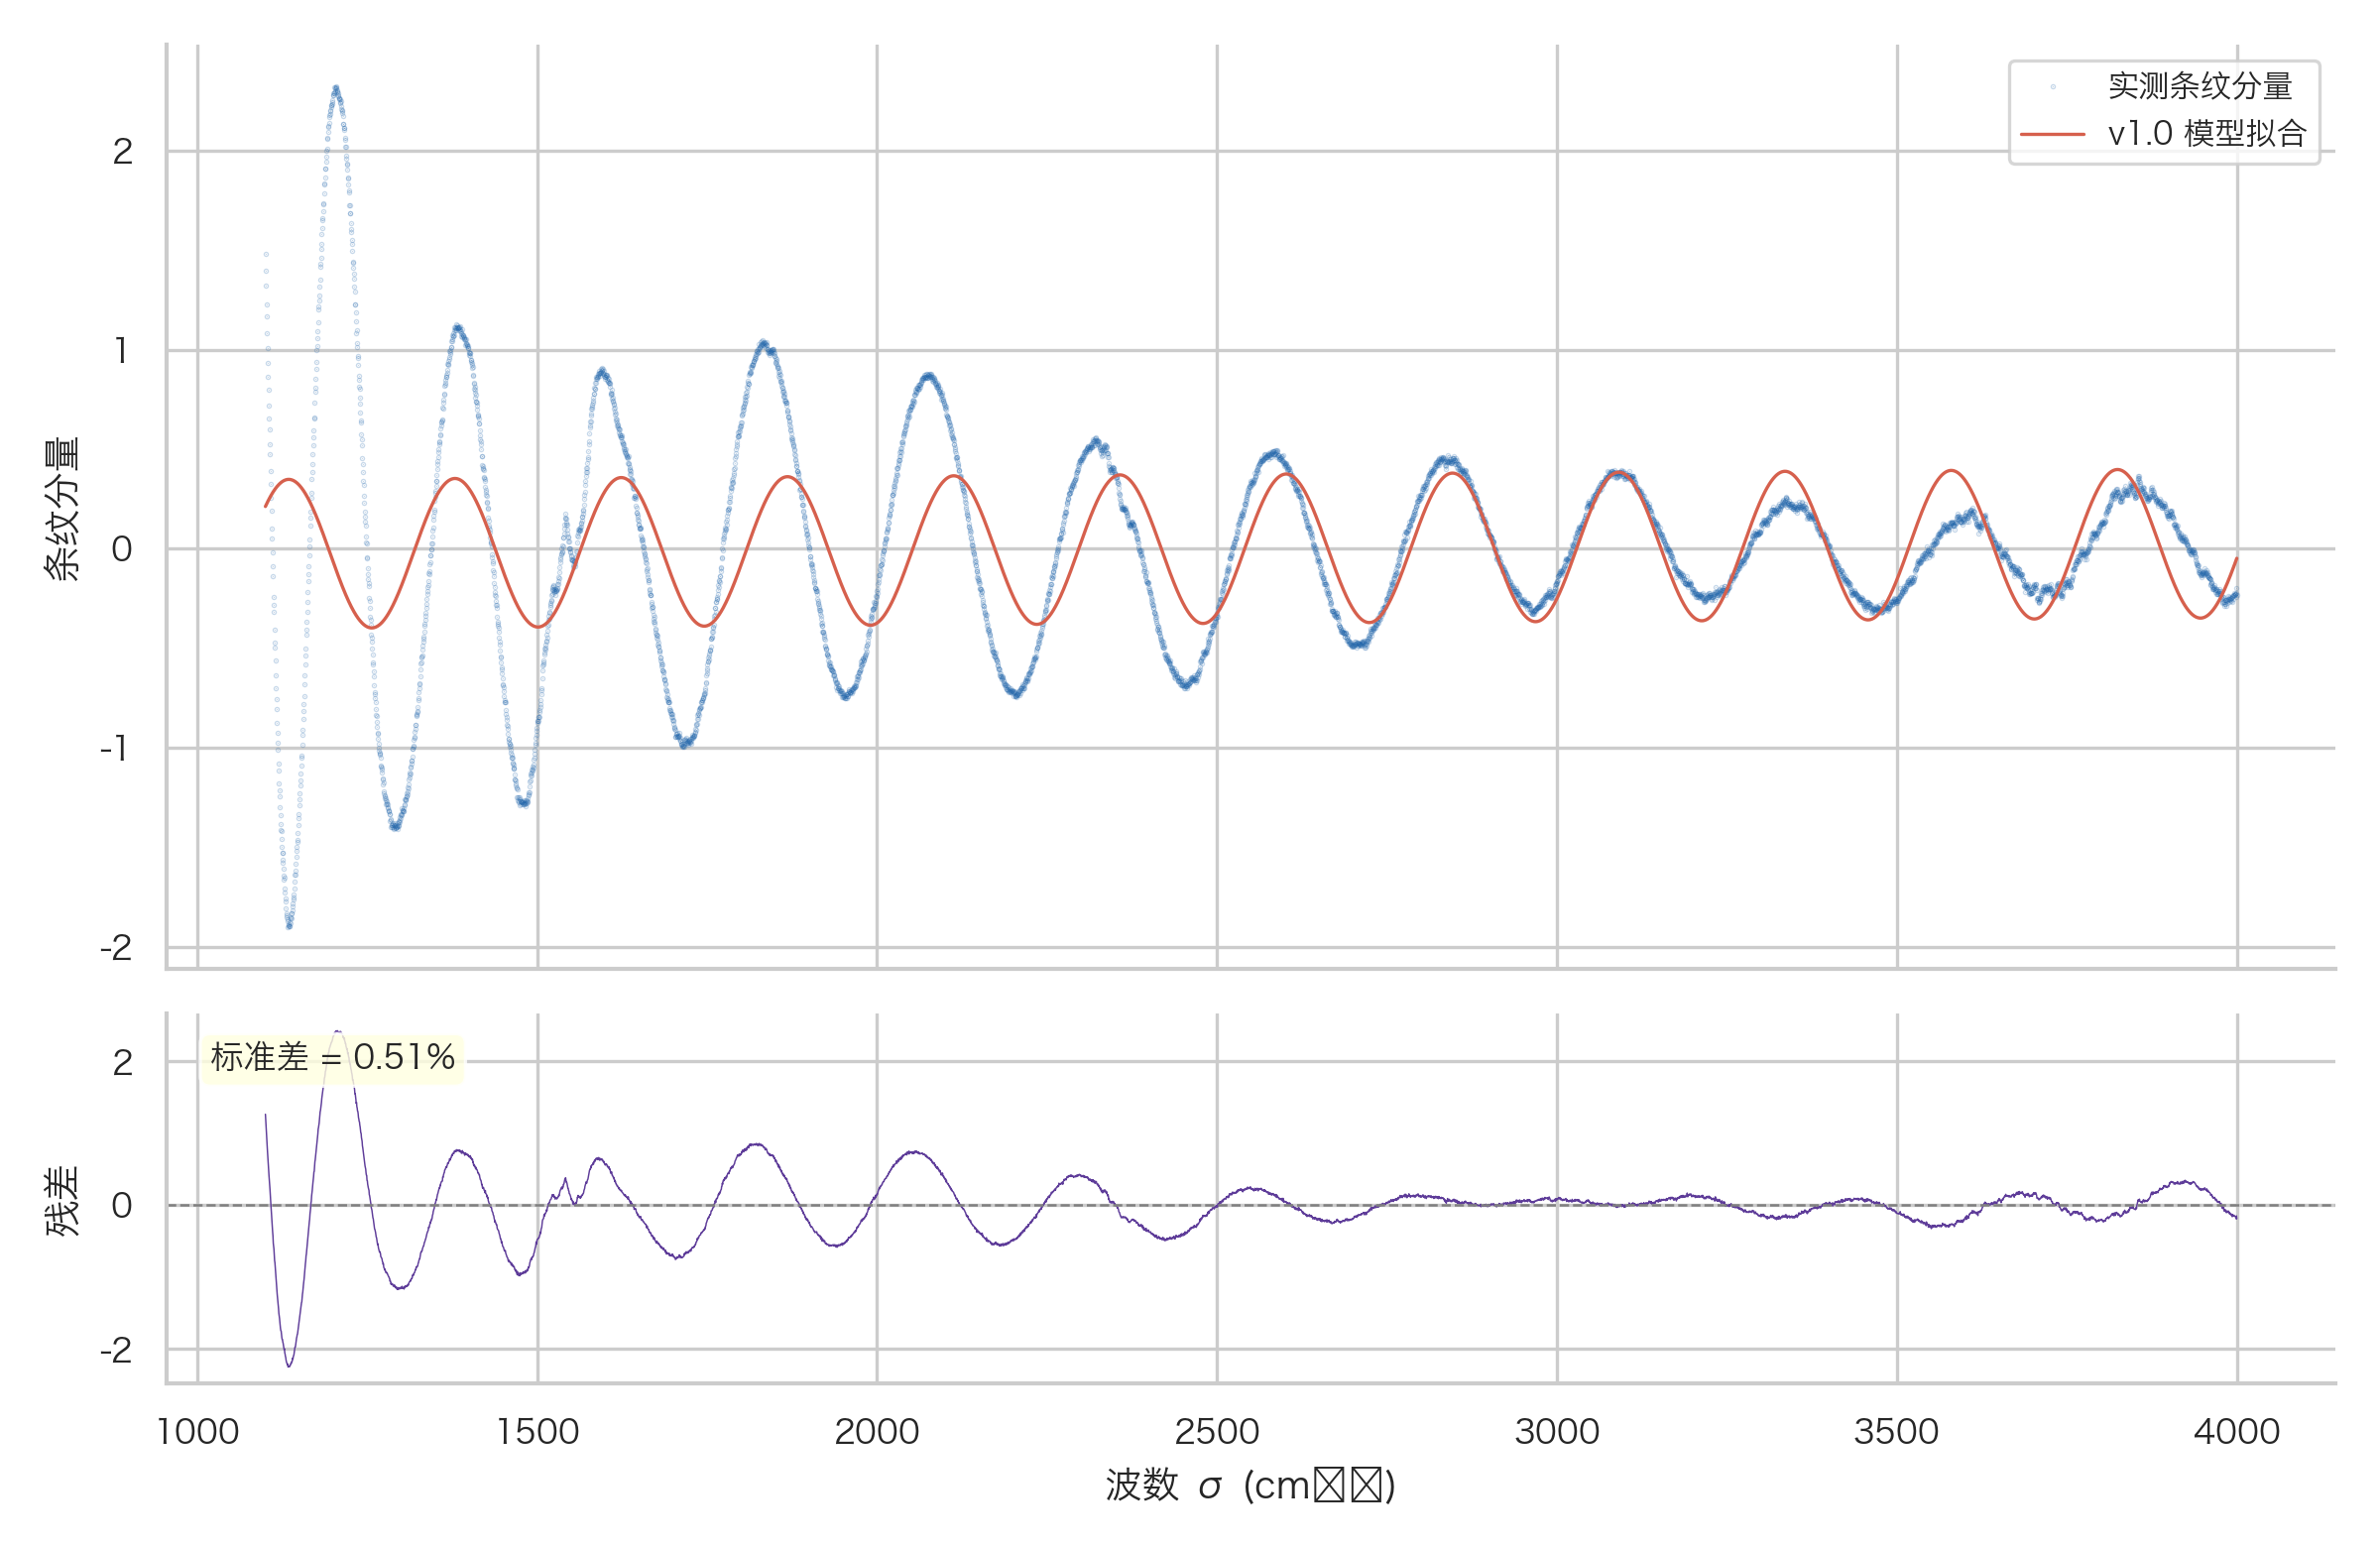
\includegraphics[width=0.9\textwidth]{../../03_结果与图表/最终图表/fig3_fitresidual.png}
  \caption{全谱拟合（v1.0 双光束模型）与残差}
  \label{fig:fig3}
\end{figure}

图\ref{fig:fig4} 为多算法交叉对照图，展示了 6 个独立估计及其误差棒，以及系统区间带 $[8.0, 8.9]\,\mu$m 和融合中心线 8.03\,$\mu$m。

\begin{figure}[H]
  \centering
  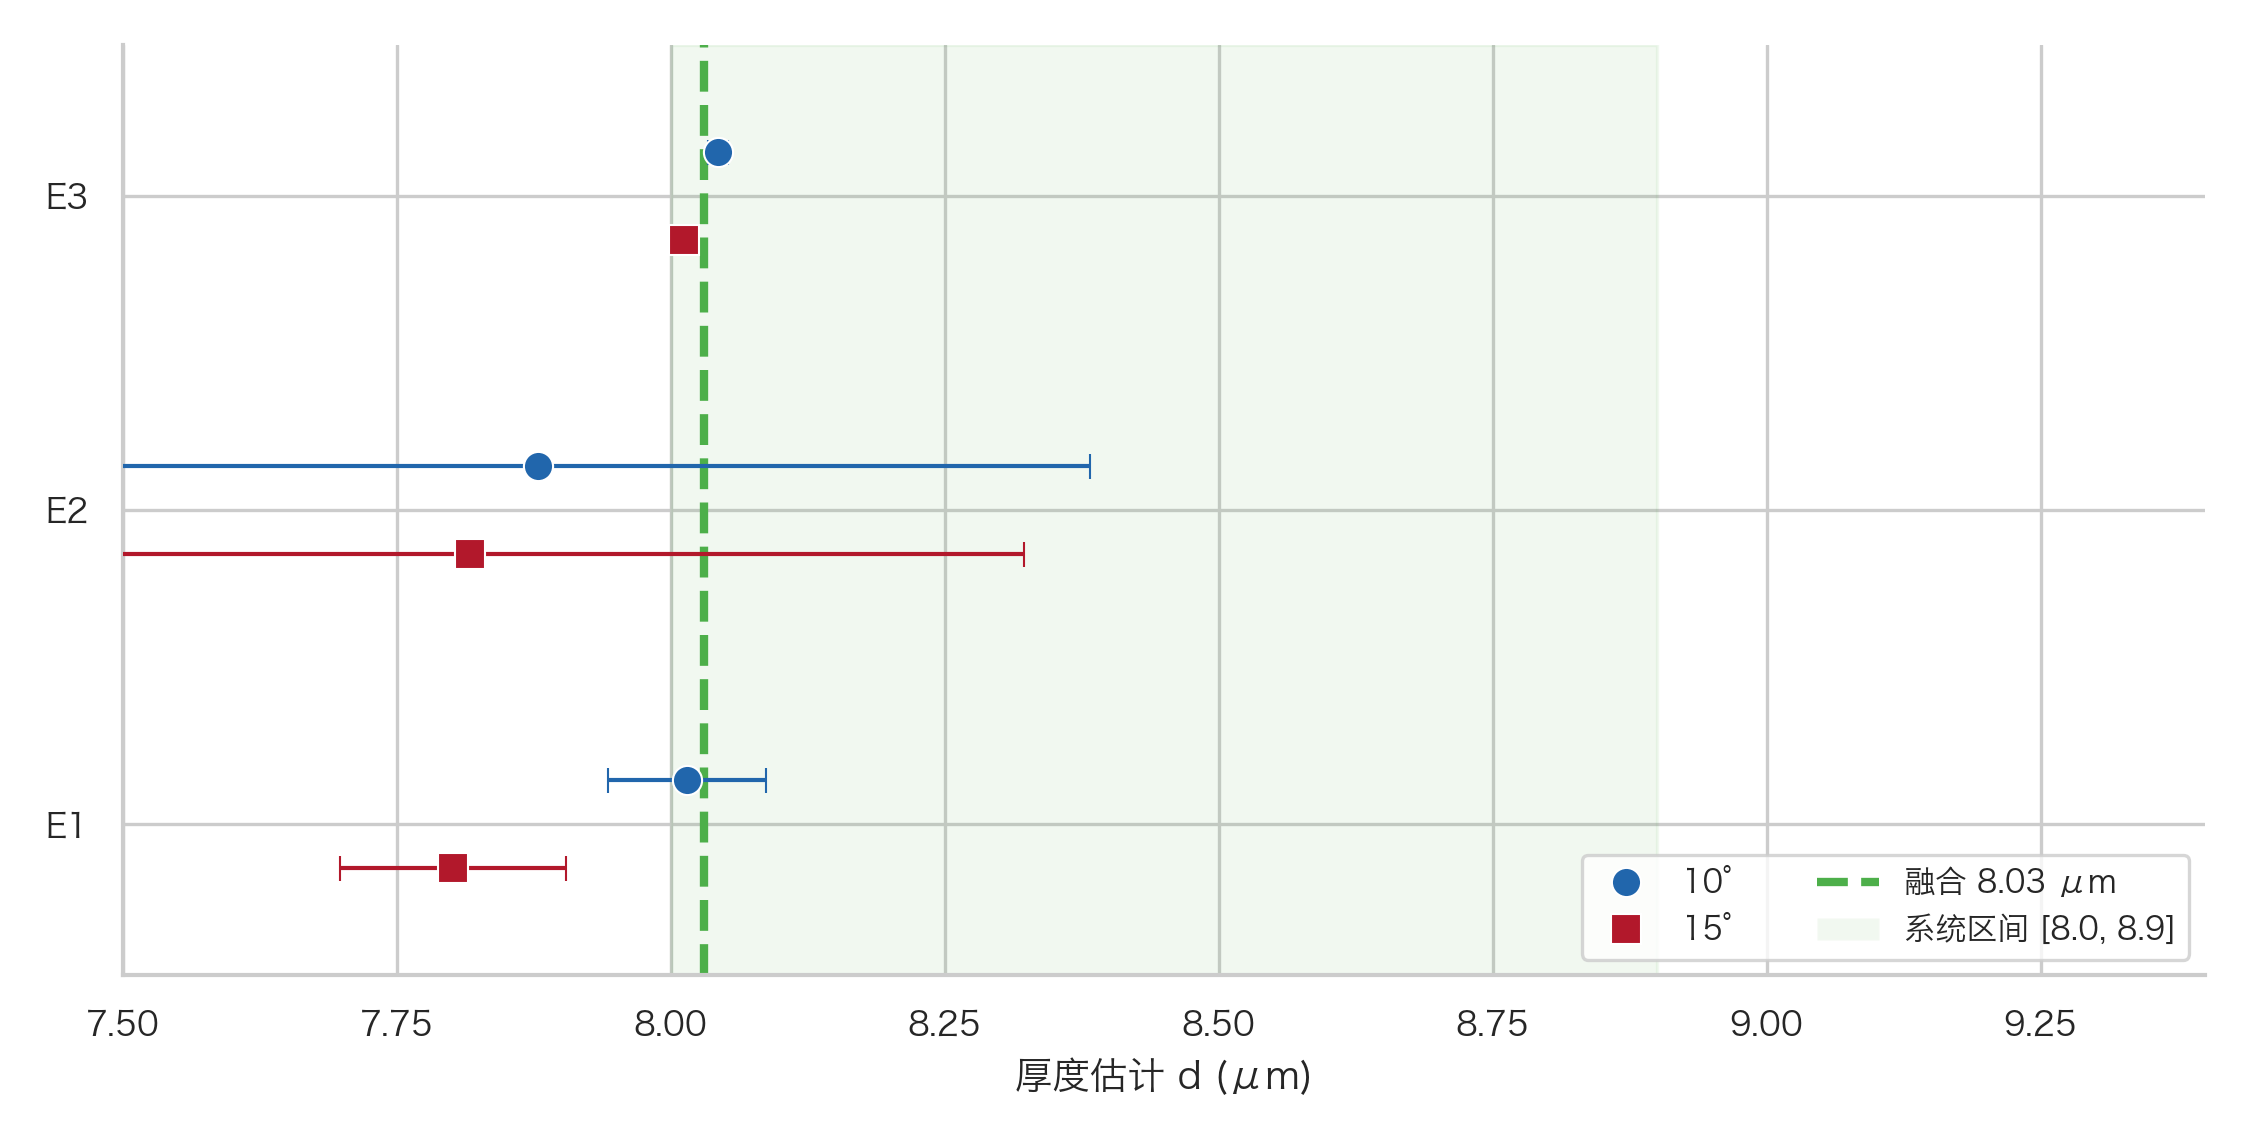
\includegraphics[width=0.95\textwidth]{../../03_结果与图表/最终图表/fig4_crosscomparison.png}
  \caption{多算法厚度估计交叉对照与系统区间}
  \label{fig:fig4}
\end{figure}

图\ref{fig:dual_angle} 为 SiC 样品两个入射角在 1800--2100\,cm$^{-1}$ 窗口的条纹分量对比，可直观看出双角度间的微小相位差（对应厚度差约 0.031\,$\mu$m，0.4\%）。

\begin{figure}[H]
  \centering
  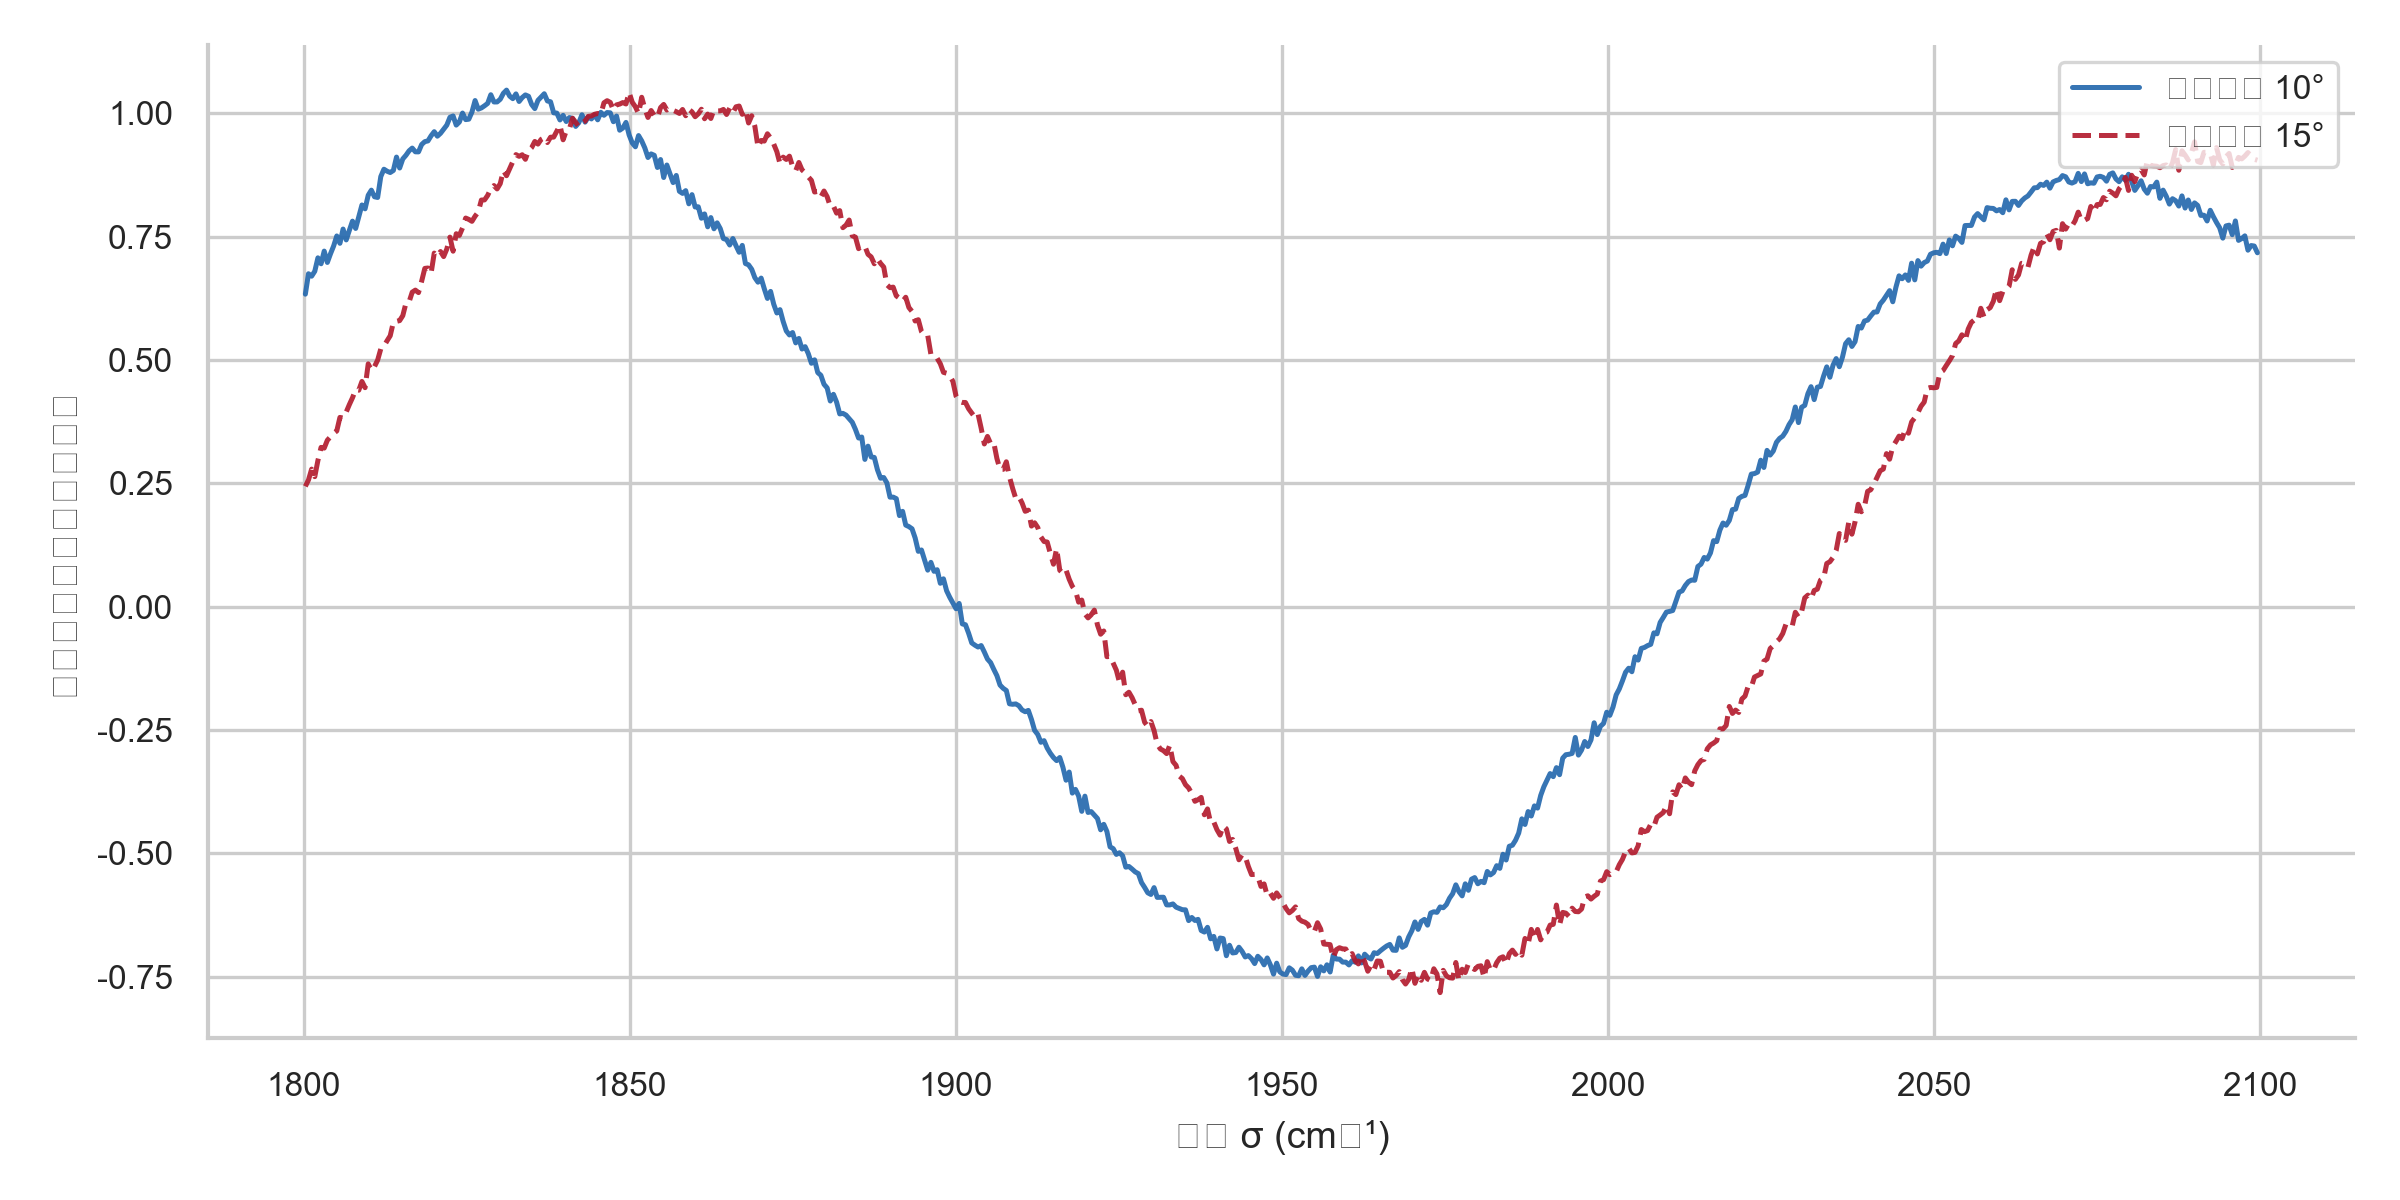
\includegraphics[width=0.88\textwidth]{../../03_结果与图表/最终图表/figC_dual_angle.png}
  \caption{双角度条纹分量对比（1800--2100\,cm$^{-1}$）}
  \label{fig:dual_angle}
\end{figure}

\subsubsection{结果合理性}

结果落在 GB/T 42905--2023 适用厚度区间（$3\sim200\,\mu$m）和工业漂移层典型区间（$5\sim30\,\mu$m）内，与 1200V 级 SiC MOSFET 漂移层（$\sim10\,\mu$m）同量级，通过合理性锚点检查。